\documentclass{report}

\usepackage[utf8]{inputenc}

\usepackage[margin=0.75in]{geometry}
\usepackage[titletoc,title]{appendix}

% Odkomentuj by zmienić tytuł abstraktu
% \renewcommand{\abstractname}{Podsumowanie}

% Wcięcie pierwszego paragrafu po rozpoczęciu sekcji, inaczej wygląda dziwnie tbh
\usepackage{indentfirst}

% Matematyka
% https://www.overleaf.com/learn/latex/Mathematical_expressions
% https://en.wikibooks.org/wiki/LaTeX/Mathematics
\usepackage{amsmath,amsfonts,amssymb,mathtools,amsthm,empheq,mathabx}

\usepackage{polski}
\numberwithin{equation}{section}

\usepackage[figurename=Fig.]{caption}
\usepackage{fancyhdr}
\usepackage{enumitem}
\usepackage[ocgcolorlinks]{hyperref}
\hypersetup{
    ocgcolorlinks=true,
    linkcolor=blue!50!red,
    urlcolor=blue!70!black
}

% Obrazki i wykresy
% https://www.overleaf.com/learn/latex/Inserting_Images
% https://en.wikibooks.org/wiki/LaTeX/Floats,_Figures_and_Captions
\usepackage{tikz}
\usepackage{graphicx,float,pgfplots,float}
\pgfplotsset{compat=newest}
\usetikzlibrary{decorations.markings}
\graphicspath{ {./images/} }
% Algorytmy
% https://www.overleaf.com/learn/latex/algorithms
% https://en.wikibooks.org/wiki/LaTeX/Algorithms
\usepackage[ruled,vlined]{algorithm2e}
\usepackage{algorithmic}

% Wyświetlanie SVG, wymaga Inkscape'a
% \usepackage{svg}
% Syntax highlighting
% https://www.overleaf.com/learn/latex/Code_Highlighting_with_minted
\usepackage{minted}
\usemintedstyle{borland}
\renewcommand{\chaptername}{Zadanie}
\def\chapterautorefname{Zadanie}

\title{WCYB Projekt 2}
\author{Jakub Bliźniuk}
\date{January 2023}


\begin{document}
\pagestyle{fancy}
\fancyfoot{}
\fancyfoot[C]{\thepage}
\fancyfoot[R]{324904}

\begin{titlepage}
    \vfill
    \maketitle
    \thispagestyle{fancy}
\end{titlepage}
\tableofcontents
\thispagestyle{fancy}
\setcounter{chapter}{4}
\chapter{Serwer zdalny VPN}
\section{Wybrana technologia VPN}
Jako preferowaną technologię wybrałem \href{https://tailscale.com}{Tailscale}\footnote{Tailscale to oparta o Wireguard sieć overlay. Cały produkt składa się z SaaS w postaci serwera kontrolnego i "awaryjnej" sieci przez którą routowany jest ruch w przypadku (rzadkiego) niepowodzenia przebicia się przez NAT/firewall, oraz aplikacji klienckich. Więcej szczegółów można znaleźć pod \url{https://tailscale.com/}}, z self-hostowanym serwerem kontrolnym - \href{https://github.com/juanfont/headscale}{Headscale}\footnote{Headscale to otwartoźródłowa wersja serwera kontrolnego Tailscale utrzymywana przez społeczność i pracowników Tailscale w ich wolnym czasie. Można ją znaleźć pod \url{https://github.com/juanfont/headscale}}. Jest to w zasadzie technologia \textit{overlay networking}, pozwalająca na dynamiczne tworzenie połączeń między urządzeniami w sieci z użyciem Wireguard.

Konfiguracja była więc podzielona na trzy części:
\begin{enumerate}
    \item Konfiguracja serwera kontrolnego, który zarządza siecią, autoryzuje połączenia i uwierzytelnia węzły
    \item Konfiguracja węzła wychodzącego, w tym wypadku na tym samym urządzniu co serwer kontrolny
    \item Zalogowanie się do sieci w aplikacji Tailscale na urządzeniach końcowych
\end{enumerate}

Dodatkowo sieć została wykorzystana w kolejnym realizowanym zadaniu (\autoref{chap:pihole}), co wymagało tylko jednej zmiany w konfiguracji urządzeń wykorzystanych w tym zadaniu.

\section{Przygotowanie maszyny wirtualnej}
Na potrzebę tego zadania stworzona została jedna maszyna wirtualna w Oracle Cloud Infrastructure (OCI) o następującej specyfikacji:
\begin{itemize}
    \item 1 rdzeń ARM Ampere Altra
    \item 6 GB RAM
    \item 1 gigabitowa karta sieciowa
    \item dysk 47GB (domyślny i jednocześnie minimalny rozmiar)
    \item system Oracle Linux (bazowany na RHEL)
\end{itemize}
Wygenerowany w OCI plik Terraform z którego ta maszyna została stworzona - z usuniętymi informacjami unikalnymi do użytego konta (identyfikator OCID sieci i projektu, klucz publiczny SSH) - znajduje się w \href{https://github.com/oplik0/WCYB-Projekt-2}{repozytorium projektu}\footnote{Link do pliku w repozytorium: \url{https://github.com/oplik0/WCYB-Projekt-2/blob/main/wcyb-machine.tf}}

\section{Konfiguracja Headscale}

W celu skonfigurowania serwera kontrolnego na Linuxie wystarczy podążałem za \href{https://github.com/juanfont/headscale/blob/main/docs/running-headscale-linux.md}{instrukcjami z repozytorium Headscale}. Kolejne kroki wyglądały następująco:

\subsection{Przygotowanie plików}

\subsubsection{Pobranie Headscale}

Headscale kompiluje się do jednego pliku wykonywalnego, który wystarczy pobrać z  ich GitHuba

\begin{minted}{bash}
wget --output-document=/bin/headscale \
https://github.com/juanfont/headscale/releases/download/v0.18.0-beta2/headscale_0.18.0-beta2_linux_arm64
\end{minted}

Warto też sprawdzić sumę kontrolną z opublikowanymi, co można zrobić komendą \mintinline{bash}{sha256sum}, co w przypadku \mintinline{go}{0.18.0-beta2} powinno wyglądać tak:

\begin{minted}{bash}
$ sha256sum /bin/headscale
e5d453352bc06fb1ffd6a16f973b40311f924e52006fe3c7d4ee227535a4153f  /bin/headscale
\end{minted}

Następnie należy upewnić się, że plik jest wykonywalny

\begin{minted}{bash}
sudo chmod +x /bin/headscale
\end{minted}

\subsection{Przygotowanie użytkownika i reszty plików}

\subsubsection{Folder na konfigurację}

Następnie należy stworzyć folder który będzie wykorzystywany do konfiguracji Headscale

\begin{minted}{bash}
sudo mkdir -p /etc/headscale
\end{minted}

\subsubsection{Stworzenie użytkownika}

W tym momencie można też już stworzyć użytkownika do usługi, co pozwoli nam też od razu stworzyć folder na dane zmienianie w czasie działania programu
\begin{minted}{bash}
sudo useradd \
	--create-home \
	--home-dir /var/lib/headscale/ \
	--system \
	--user-group \
	--shell /usr/bin/nologin \
	headscale    
\end{minted}

\subsubsection{Stworzenie pustego pliku bazy danych}

\begin{minted}{bash}
    sudo -u headscale touch /var/lib/headscale/db.sqlite
\end{minted}

\subsubsection{Stworzenie pliku konfiguracyjnego}

Możemy w tym momencie stworzyć też pusty plik konfiguracyjny, ale prościej jest zacząć od \href{https://github.com/juanfont/headscale/blob/main/config-example.yaml}{przykładowej konfiguracji z repozytorium Headscale}\footnote{\url{https://github.com/juanfont/headscale/blob/main/config-example.yaml}} - najprościej to zrobić po prostu przeklejając tekst z użyciem preferowanego edytora tekstu

\begin{minted}{bash}
sudoedit /etc/headscale/config.yaml
\end{minted}

Można już też w tym momencie edytować konfigurację - ostateczna wersja z którą skończyłem (z usuniętymi identyfikatorami i sekretem OpenID Connect) znajduje się w \href{https://github.com/oplik0/WCYB-Projekt-2/blob/main/config.yaml}{Repozytorium projektu}\footnote{Link do pliku: \url{https://github.com/oplik0/WCYB-Projekt-2/blob/main/config.yaml}}

\subsubsection{Konfiguracja ACL}
Domyślnie każdy użytkownik ma dostęp tylko do swoich urządzeń. Można jednak to zmienić, a także pozwolić wykonywać połączenia poza sieć wirtualną, ustawiając listy kontroli dostępu. Wykorzystana przeze mnie konfiguracja pobiera listy z pliku \mintinline{bash}{/etc/headscale/acl.jsonc}. Kopia wykorzystanego przeze mnie pliku znajduje się w \href{https://github.com/oplik0/WCYB-Projekt-2/blob/main/acl.jsonc}{repozytorium projektu pod nazwą \mintinline{bash}{acl.jsonc}}\footnote{Link do pliku ACL: \url{https://github.com/oplik0/WCYB-Projekt-2/blob/main/acl.jsonc}}
\begin{samepage}
\subsection{Konfiguracja usługi}
W tym momencie headscale powinno już działać, co można sprawdzić komendą \mintinline{bash}{headscale serve} - lepszym pomysłem niż manualne uruchamianie jest jednak stworzenie usługi SystemD - co możemy zrobić tworząc plik \mintinline{bash}{/etc/systemd/system/headscale.service}, np. używając edytora przez \mintinline{bash}{sudoedit /etc/systemd/system/headscale.service}.
Zawartość pliku powinna wyglądać następująco:
\begin{minted}{ini}
[Unit]
Description=headscale controller
After=syslog.target
After=network.target

[Service]
Type=simple
User=headscale
Group=headscale
ExecStart=/bin/headscale serve
Restart=always
RestartSec=5

# Optional security enhancements
NoNewPrivileges=yes
PrivateTmp=yes
ProtectSystem=strict
ProtectHome=yes
ReadWritePaths=/var/lib/headscale /var/run/headscale
AmbientCapabilities=CAP_NET_BIND_SERVICE
RuntimeDirectory=headscale

[Install]
WantedBy=multi-user.target
\end{minted}
\end{samepage}

\subsection{Otwieranie portów w firewallu}
\subsubsection{Otworzenie gRPC i STUN}
Headscale wystawia usługi na kilku potrach. W konfiguracji z którą skończyłem dwie z nich powinny być wystawione do internetu - gRPC i STUN. Możemy je przepuścić na serwerze komendą \mintinline{bash}{firewall-cmd}:
\begin{minted}{bash}
sudo firewall-cmd --add-port=50443/tcp --permanent
sudo firewall-cmd --add-port=3478/tcp --permanent
sudo firewall-cmd --reload
\end{minted}
Przez wykorzystanie Oracle Cloud Infrastructure należało te porty przepuścić też na listach bezpieczeństwa w sieci wirtualnej w OCI, co jednak zrobiłem wcześniej.
\subsubsection{Otworzenie portów HTTP(S)}
Tailscale do kontroli wykorzystuje też protokół HTTP(S). Konfiguracja Tailscale nie wystawia go na zewnątrz - zmiast tego posłuży do tego serwer nginx, co pozwoli też dodać statyczną stronę do zarządzania serwerem (korzystając z projektu \href{https://github.com/gurucomputing/headscale-ui}{headscale-ui}). Ponownie robimy to z pomocą \mintinline{bash}{firewall-cmd}, tym razem jednak istnieją już predefiniowane usługi:
\begin{minted}{bash}
sudo firewall-cmd --add-service=http --permanent
sudo firewall-cmd --add-service=https --permanent
sudo firewall-cmd --reload
\end{minted}
\subsection{Uruchomienie usługi}
Ostatnim krokiem jest uruchomienie Headscale i sprawdzenie czy działa. Wystarczy do tego przeładować usługi systemd i włączyć stworzoną wcześniej usługę:
\begin{minted}{bash}
sudo systemctl daemon-reload
sudo systemctl enable --now headscale
\end{minted}
Możemy teraz sprawdzić status usługi komendą \mintinline{bash}{systemctl status headscale} i upewnić się, że wszystko działa poprwnie sprawdzając wystawione metryki z użyciem \mintinline{bash}{curl http://127.0.0.1:9090/metrics}

\section{Headscale-UI i nginx}

Jednym elementem którego brakuje w Headscale w stosunku do oferty SaaS jest panel administratora. Istnieje jednak osobny projekt adresujący tę potrzebę, nawet jeśli nie jest jeszcze na poziomie oficjalnego rozwiązania. \href{https://github.com/gurucomputing/headscale-ui}{Headscale-UI} jest prostą stroną statyczną napisaną w SvelteKit. Możemy ją serwować wykorzystując nginx jako proxy do zarówno headscale jak i panelu, wystawiając je pod tą samą domeną.

\subsection{Pobranie Headscale-UI}

W repozytorium projektu jako wydania publikowane są pliki zip zawierające zbudowaną wersję strony. Możemy więc dość łatwo pobrać projekt i go rozpakować do \mintinline{bash}{/srv}:
\begin{minted}{bash}
wget --output-document=/srv/headscale-ui.zip \
https://github.com/gurucomputing/headscale-ui/releases/download/2022.12.23.2-beta/headscale-ui.zip

unzip /srv/headscale-ui.zip
\end{minted}
Przez wykorzystanie SELinuxa w Oracle Linux należy też odpowiednio oznaczyć pliki by nginx miał do nich później dostęp:
\begin{minted}{bash}
semanage fcontext -a -t httpd_sys_content_t "/srv/headscale-ui(/.*)?"
restorecon -Rv /srv/headscale-ui
\end{minted}
\subsection{Instalacja nginx}

W przypadku Oracle Linux nginx należy zainstalować korzystając z menadżera pakietów \mintinline{bash}{dnf} (lub starszego \mintinline{bash}{yum}). Inne dystrybucje mogą używać innych menedżerów pakietów (np. \mintinline{bash}{apt} w Debianie/Ubuntu):

\begin{minted}{bash}
sudo dnf install nginx
\end{minted}

Przy okazji można też zainstalować narzędzie certbot które można wykorzystać do wygenerowania certyfikatów dla domeny na której będzie serwowana strona i headscale:

\begin{minted}{bash}
sudo dnf install certbot python3-certbot-nginx
\end{minted}

\begin{samepage}    
\subsection{Konfiguracja nginx}
Następnie należy stworzyć konfigurację nginx - to co ważne to zdefiniowane dwóch bloków \mintinline{bash}{location}:
\begin{minted}{yaml}
    location /web {
            alias /srv/headscale-ui/;
            index index.html;
    }
    location / {
        proxy_pass http://127.0.0.1:8080;
        proxy_http_version 1.1;
        proxy_set_header Upgrade $http_upgrade;
        proxy_set_header Connection $connection_upgrade;
        proxy_set_header Host $server_name;
        proxy_redirect http:// https://;
        proxy_buffering off;
        proxy_set_header X-Real-IP $remote_addr;
        proxy_set_header X-Forwarded-For $proxy_add_x_forwarded_for;
        proxy_set_header X-Forwarded-Proto $http_x_forwarded_proto;
        add_header Strict-Transport-Security "max-age=15552000; includeSubDomains" always;
    }
\end{minted}
Ostateczna konfiguracja z którą skończyłem, po dodatkowym wykorzystaniu narzędzia certbot w celu wygenerowania certyfikatów TLS dla domeny, znajduje się w \href{https://github.com/oplik0/WCYB-Projekt-2/blob/main/headscale.conf}{repozytorium projektu jako headscale.conf}\footnote{Link do pliku: \url{https://github.com/oplik0/WCYB-Projekt-2/blob/main/headscale.conf}}
\end{samepage}

\subsection{Uruchomienie nginx}

Po skonfigurowaniu wystarczy włączyć usługę:
\begin{minted}{bash}
sudo systemctl enable --now nginx
\end{minted}

\subsection{pobranie klucza API}
By móc połączyć panel administracyjny z API Headscale należy wygenerować klucz na serwerze używając komendy
\begin{minted}{bash}
headscale apikeys create
\end{minted}
Po wklejeniu go w ustawieniach panelu zostanie on zapisany lokalnie w przeglądarce (krok ten trzeba więc powtarzać na każdym urządzeniu), co pozwoli nam zarządzać użytkownikami i urządzeniami.

\section{Konfiguracja Tailscale na serwerze (exit-node)}
\subsection{Instalacja Tailscale}
By zainstalować klienta Tailscale wystarczy podążyć za instrukcjami dla wybranej dystrybucji na stronie Tailscale, w tym wypadku dla Oracle Linux będzie to: \url{https://tailscale.com/download/linux/oracle-linux-8}
\subsubsection{Dodanie repozytoriów i instalacja}
\begin{minted}{bash}
sudo dnf config-manager --add-repo https://pkgs.tailscale.com/stable/oracle/8/tailscale.repo
sudo dnf install tailscale
\end{minted}
\subsubsection{Właczenie usługi}
\begin{minted}{bash}
sudo systemctl enable --now tailscaled
\end{minted}
\subsubsection{Pozwolenia na masquarade w firewalld}
Ta część jest wymagana by móc przepuścić ruch klientów przez serwer do internetu
\begin{minted}{bash}
firewall-cmd --permanent --add-masquerade
\end{minted}
\subsection{Połączenie z siecią}
Po zainstalowaniu wystarczy wykonać jedną komendę do połączenia się z siecią tailscale:
\begin{minted}
tailscale up --login-server=https://wcyb.blizni.uk --advertise-exit-node --advertise-tags=tag:common,tag:admin
\end{minted}
Parametr \mintinline{bash}{--login-server} definiuje serwer kontrolny, \mintinline{bash}{--advertise-exit-node} pozwala innym urządzeniom łączyć się przez to do internetu, a \mintinline{bash}{--advertise-tags} ustawia tagi, które wg. zdefiniowanych wcześniej ACL pozwalają połączyć się z tą maszyną.

Po wykonaniu komenda ta powinna przekierować do dostawcy OIDC w celu zalogowania się. Jeśli nie jest to skonfigurowane należy zamias tego stworzyć użytkownika w headscale-ui i stworzyć dla niego Preauth Key który należy dodać w parametrze \mintinline{bash}{--auth-key}

\section{Konfiguracja klienta}
Ostatnią częścią zadania jest skonfigurowanie klienta (w tym wypadku Windows), co jest nawet prostsze niż w przypadku serwera.
\subsection{Pobranie tailscale}
Wystarczy pobrać instalator ze strony \url{https://tailscale.com/download/windows}, uruchomić go i podążać za krokami instalacji.
\subsection{Logowanie}
Z powodu użycia innego serwera po uruchomieniu aplikacji zamiast wybrania "Log In" w tacy systemowej należy otworzyć terminal (Powershell/CMD) i wykonać podobną komendę jak na serwerze:
\begin{minted}{powershell}
tailscale up --login-server=https://wcyb.blizni.uk
\end{minted}
Nie potrzebujemy tu jednak reklamować węzła wyjściowego ani tagów.

Podobnie jak w przypadku serwera, jeśli nie mamy konfiguracji OIDC należy stworzyć preauth key w headscale-ui.
\section{Podsumowanie zadania}
\subsection{Sprawdzenie działania}
Możemy teraz połączyć się przez węzeł wyjściowy korzystając z odpowiedniej opcji w tacy systemowej. Możemy potwierdzić topologię sieci korzystając z komendy \mintinline{powershell}{tailscale status} (fig. \ref{fig:tailscale_status})
\begin{figure}[H]
    \centering
    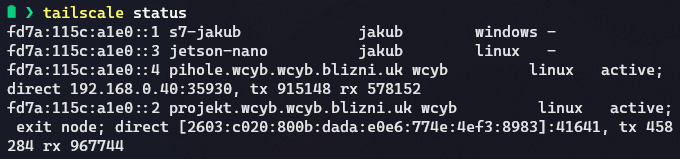
\includegraphics[scale=1]{tailscale-status.png}
    \caption{Status tailscale}
    \label{fig:tailscale_status}
\end{figure}
\begin{samepage}
A także potwierdzić, że nasz adres IP to adres serwera korzystając np. z DuckDuckGo (fig. \ref{fig:ip_check}):
\begin{figure}[H]
    \centering
    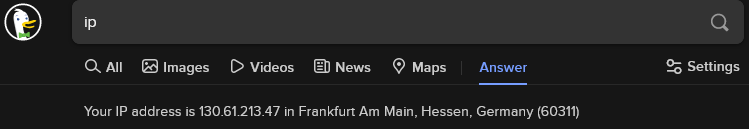
\includegraphics[scale=0.5]{ddg-ip.png}
    \caption{Obecne IP wg. DuckDuckGo}
    \label{fig:ip_check}
\end{figure}
Co jak widać zwraca adres z Frankfurtu, w którym obecnie się nie znajduję.
\end{samepage}
\subsection{Wnioski}
Najdłuższą częścią tego projektu (pomijając walkę z Oktą, która tutaj została bardzo delikatnie wspomniana) było pisanie tego raportu, co pokazuje jak prosto jest obecnie skonfiguorwać sensowną sieć wirtualną na własny użytek. Tailscale pozwala nie tylko na wykorzystanie serwera jako krok między komputerem a internetem, ale daje możliwość dostępu do urządzeń gdziekolwiek by nie były praktycznie tak samo łatwo jakby były w sieci lokalnej (a jak nawet widać na fig. \ref{fig:tailscale_status} w przypadku dwóch urządzeń lokalnych połaczenie nawet nie wyjdzie przez internet), bez żadnego pośrednika. Zresztą poza wystawianiem internetu, istnieje możliwość reklamowania sieci lokalnej dając przez jeden "router brzegowy" dostęp do wszystkiego co się w niej znajduje w tailscale (co realizowało by drugą opcję projektu).

Na razie poza ideologiczną chęcią utrzymania kontroli lub specyficznymi wymaganiami nie widzę jednak sensu utrzymywania serwera kontrolnego przy hojnej darmowej ofercie SaaS, więc sam wrócę do tego rozwiązania po projekcie.
\chapter{PiHole}
\label{chap:pihole}
\end{document}
